\documentclass[11pt,a4paper]{article}
\usepackage[T1]{fontenc}
\usepackage[utf8]{inputenc}
\usepackage[french]{babel}
\usepackage[margin=2.4cm]{geometry}
\usepackage{lmodern}
\usepackage{amsmath,amssymb}
\usepackage{graphicx}
\usepackage{booktabs}
\usepackage{microtype}
\usepackage{xcolor}
\usepackage[hidelinks]{hyperref}
\usepackage{enumitem}
\setlist{itemsep=3pt,topsep=5pt}
\setlength{\parskip}{5pt}
\setlength{\parindent}{0pt}
\graphicspath{{figures/}{rapport/figures/}}

\title{Do flat minima generalize better?\\[0.3em]
\large Rapport d'avancement du projet HDDL}
\author{Projet HDDL}
\date{27 novembre 2026}

\begin{document}
\maketitle

\begin{abstract}
Ce projet cherche à étudier expérimentalement le lien entre la forme de la fonction de coût autour des poids d'un réseau et sa capacité à généraliser. Une première expérience a été réalisée avec un petit réseau de classification et trois tailles de batch. La sensibilité des solutions est estimée en perturbant les poids et en mesurant la variation de la fonction de coût. Les premiers résultats montrent une association entre une moindre sensibilité et une meilleure précision test dans ce protocole. Ils ne permettent toutefois pas de conclure que la platitude en est la cause, car les modèles n'ont pas atteint le même niveau d'apprentissage. Ce rapport présente le travail réalisé et les comparaisons prévues pour approfondir cette question.
\end{abstract}

\section{Problématique}

Un réseau de neurones est entraîné en ajustant ses paramètres pour réduire une fonction de coût, appelée \emph{loss}. Une faible erreur sur les exemples d'entraînement ne suffit cependant pas : on souhaite aussi obtenir de bonnes prédictions sur des exemples qui n'ont pas servi à ajuster les paramètres. C'est la question de la généralisation.

Le sujet du projet est le suivant : \emph{les minima plats généralisent-ils mieux ?} Intuitivement, une région est dite plate lorsque de petites modifications des poids changent peu la loss. À l'inverse, une région plus pointue est sensible à ces modifications. L'hypothèse étudiée est qu'une solution moins sensible pourrait mieux se comporter sur des données nouvelles.

Cette intuition doit être testée. Une robustesse aux perturbations des poids et une bonne performance sur des données nouvelles sont deux propriétés différentes. Nous ne supposerons donc pas que l'une implique automatiquement l'autre. De plus, les poids obtenus à la fin d'un entraînement ne sont pas nécessairement un minimum local : nous parlerons de \emph{solutions obtenues} lorsque cette distinction est utile.

L'objectif est de construire une expérience assez simple pour comprendre chaque étape, puis d'améliorer progressivement le protocole. Il ne s'agit pas, à ce stade, d'établir un résultat valable pour tous les réseaux de neurones.

\section{Notions utilisées et lien avec le cours}

\subsection{Apprentissage et généralisation}

En notant $\theta$ les paramètres du réseau, la loss d'entraînement s'écrit
\[
L_{\mathrm{train}}(\theta)
=\frac{1}{n}\sum_{i=1}^{n}\ell(f_\theta(x_i),y_i),
\]
où $f_\theta(x_i)$ représente les sorties du réseau et $\ell$ l'entropie croisée pour la classification.

On utilise deux indicateurs complémentaires : la loss et l'\emph{accuracy}, c'est-à-dire la proportion de prédictions correctes. L'écart de précision entre entraînement et test est défini par
\[
G_{\mathrm{acc}}=A_{\mathrm{train}}-A_{\mathrm{test}}.
\]
Un faible écart ne signifie pas nécessairement que le modèle est bon : un réseau qui apprend peu peut être médiocre sur les deux ensembles et présenter un faible écart. Il faut donc examiner simultanément les performances d'entraînement et de test.

Le cours sur les autoencodeurs illustre cette distinction avec un modèle qui mémoriserait chaque exemple sans pouvoir généraliser (\texttt{AE.pdf}, page 48 du fichier, diapositive 20). Cette idée sert de point de départ au projet, même si notre expérience porte sur la classification.

\subsection{Optimisation par mini-batchs}

La descente de gradient stochastique, ou SGD, met à jour les paramètres à partir d'un sous-ensemble des données :
\[
\theta_{t+1}=\theta_t-\eta\nabla_\theta L_{B_t}(\theta_t),
\]
où $B_t$ est le mini-batch courant et $\eta$ le taux d'apprentissage. La taille du batch modifie la composition des gradients utilisés et le nombre de mises à jour par époque. Elle constitue le premier paramètre que nous faisons varier.

Les exemples PyTorch du TP CNN, présents dans \texttt{5ModIA-HDDL-main.zip}, servent de référence pour l'organisation de l'entraînement : définition du modèle, calcul de la loss, optimisation et suivi des performances sur un ensemble de validation. Nous conservons ces principes avec une architecture plus petite, adaptée à une première expérience sur CPU.

\section{Protocole déjà mis en place}

\subsection{Données et modèle}

L'expérience utilise \texttt{load\_digits} de scikit-learn, qui contient 1\,797 images de chiffres manuscrits réparties en dix classes. Chaque image mesure $8\times8$ pixels. Les 64 valeurs sont divisées par 16 pour être ramenées dans l'intervalle $[0,1]$, puis fournies au réseau sous forme de vecteur.

La séparation est stratifiée, afin de conserver approximativement les proportions des classes : 1\,077 exemples pour l'entraînement, 360 pour la validation et 360 pour le test. Elle reste identique pour tous les essais, avec une graine de séparation fixée à 42.

Le réseau est un perceptron multicouche :
\[
\mathbb{R}^{64}\ \longrightarrow\ \mathrm{Linear}(64,64)
\ \longrightarrow\ \mathrm{ReLU}
\ \longrightarrow\ \mathrm{Linear}(64,10).
\]
La sortie contient dix scores, ou \emph{logits}, directement transmis à la fonction d'entropie croisée de PyTorch. Il n'est pas nécessaire d'ajouter une couche softmax dans le code du modèle.

\subsection{Entraînements réalisés}

\begin{table}[htbp]
\centering
\begin{tabular}{ll}
\toprule
Paramètre & Valeur \\
\midrule
Optimiseur & SGD sans momentum \\
Taux d'apprentissage & $0{,}1$, constant \\
Nombre d'époques & 100 \\
Tailles de batch & 16, 128 et 512 \\
Graines d'entraînement & 0, 1 et 2 \\
Nombre total d'entraînements & 9 \\
Régularisation explicite & Aucune \\
\bottomrule
\end{tabular}
\caption{Configuration de la première expérience.}
\end{table}

Pour une même graine, les trois modèles partent des mêmes poids et utilisent le même ordre de permutation des exemples à chaque époque, découpé en batchs de tailles différentes. Cela réduit certaines sources de variation entre les essais.

La loss et l'accuracy d'entraînement et de validation sont enregistrées après chaque époque. Le modèle évalué sur le test est celui de la dernière époque. Cette première version ne sélectionne pas automatiquement un modèle à partir de la validation.

\subsection{Mesure de sensibilité des poids}

La platitude est approchée par une mesure de sensibilité locale. Pour chaque tenseur de paramètres $\theta_j$, on tire un bruit gaussien $z_j$ puis on construit une perturbation relative :
\[
\delta_j(\rho)=\rho\,\|\theta_j\|_2\frac{z_j}{\|z_j\|_2}.
\]
Pour les matrices, la norme désigne la norme euclidienne de leurs coefficients, équivalente à la norme de Frobenius. La règle est appliquée aux poids et aux biais. Un tenseur de norme nulle reste inchangé.

Pour une amplitude $\rho$, la mesure calculée est
\[
S_\rho(\theta)=\frac{1}{K}\sum_{k=1}^{K}
\left[
\frac{L_{\mathrm{train}}(\theta+\delta^{(k)}(\rho))
+L_{\mathrm{train}}(\theta-\delta^{(k)}(\rho))}{2}
-L_{\mathrm{train}}(\theta)
\right].
\]
Nous utilisons $K=20$ directions et trois amplitudes : $\rho\in\{0{,}01;0{,}05;0{,}10\}$. Les mêmes directions sont réutilisées pour les différentes amplitudes d'un modèle. La moyenne des perturbations opposées limite la contribution du terme de premier ordre lorsque la loss est localement régulière.

Une faible valeur de $S_\rho$ indique une faible augmentation moyenne de la loss dans les directions testées. Il ne s'agit ni de la perturbation la plus défavorable ni d'un calcul de la Hessienne. Cette mesure dépend encore de la paramétrisation du réseau, malgré la normalisation relative du bruit. Elle ne permet donc pas de définir une notion universelle de platitude.

\section{Premiers résultats}

Les neuf entraînements ont été exécutés. Les valeurs du tableau suivant sont des moyennes sur les trois graines. Les résultats proviennent du fichier \texttt{results/results.csv}.

\begin{table}[htbp]
\centering
\small
\begin{tabular}{rrrrr}
\toprule
Batch & Accuracy train & Accuracy test & Écart (points) & $S_{0{,}05}$ \\
\midrule
16  & $100{,}0\,\%$ & $95{,}8\,\%$ & $4{,}17$ & $0{,}000717$ \\
128 & $98{,}0\,\%$  & $95{,}4\,\%$ & $2{,}65$ & $0{,}001205$ \\
512 & $93{,}8\,\%$  & $92{,}8\,\%$ & $1{,}03$ & $0{,}001259$ \\
\bottomrule
\end{tabular}
\caption{Performances finales et sensibilité aux perturbations relatives de 5\,\%. Les écarts sont calculés avant arrondi des accuracies.}
\end{table}

Le batch de 16 donne la meilleure précision test et la plus faible sensibilité moyenne. Cette observation va dans le sens de l'hypothèse étudiée, dans les limites de ce protocole. Cependant, son écart entraînement--test est aussi le plus grand. La conclusion dépend donc de ce que l'on entend par \og mieux généraliser\fg{} : obtenir une meilleure performance test ou réduire l'écart avec l'entraînement ne revient pas au même.

Les losses d'entraînement moyennes sont respectivement $0{,}0106$, $0{,}1049$ et $0{,}2901$ pour les batchs de 16, 128 et 512. Les modèles ne se trouvent donc pas au même niveau d'optimisation.

\begin{figure}[htbp]
\centering
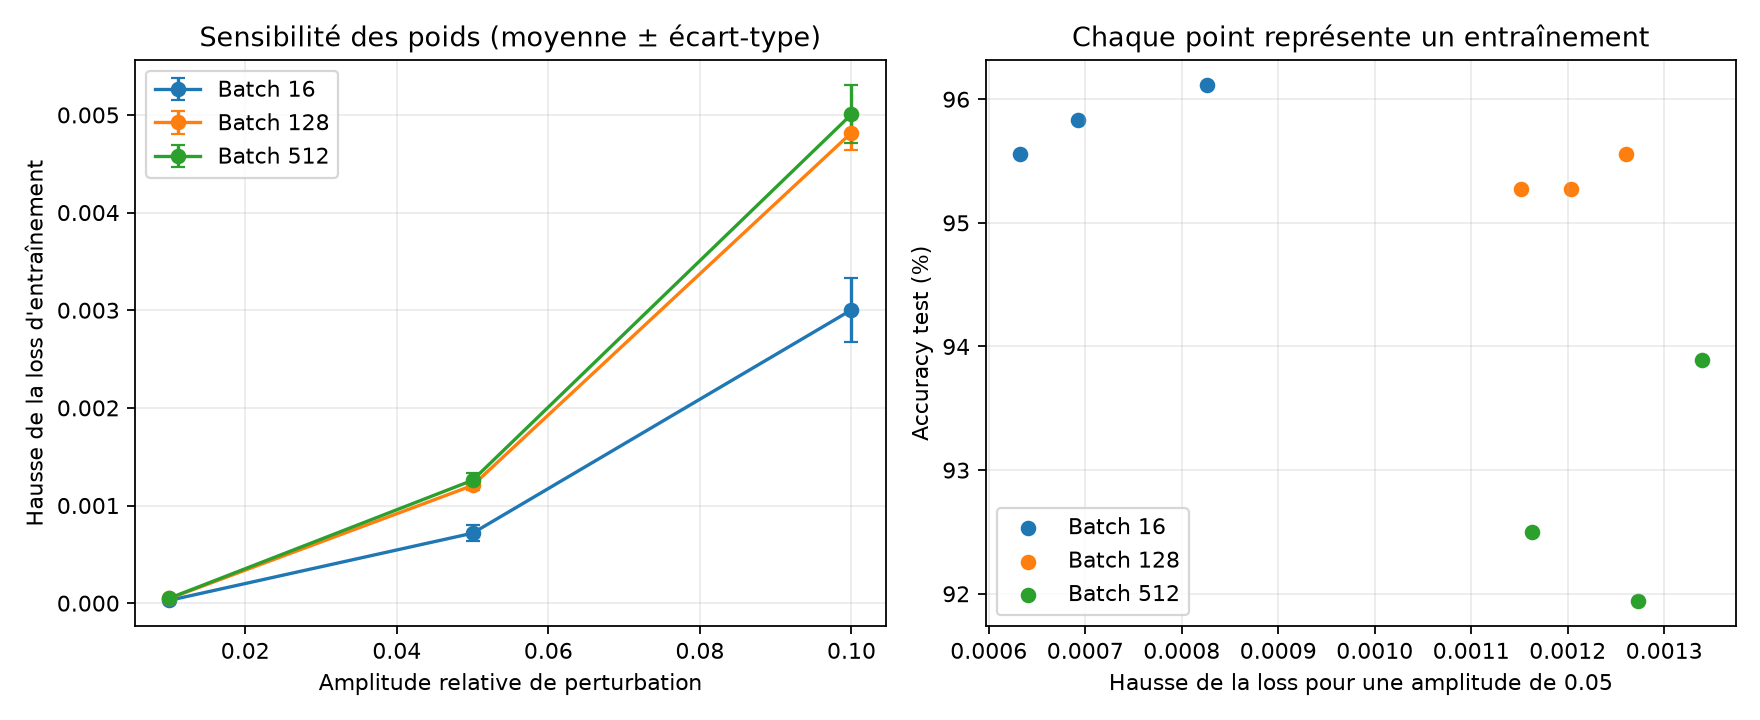
\includegraphics[width=\textwidth]{comparison.png}
\caption{À gauche, augmentation moyenne de la loss selon l'amplitude de perturbation ; les barres représentent l'écart-type entre les trois graines, pas un intervalle de confiance. À droite, sensibilité à 5\,\% et précision test ; chaque point correspond à un entraînement.}
\label{fig:results}
\end{figure}

\subsection{Limites de l'interprétation}

La principale difficulté est le budget d'optimisation. Avec 1\,077 exemples d'entraînement et 100 époques, les trois tailles de batch conduisent respectivement à 6\,800, 900 et 300 mises à jour. Le batch de 16 bénéficie donc de beaucoup plus d'étapes d'optimisation. Une meilleure performance finale ne peut pas être attribuée uniquement à une région plus plate.

Trois graines donnent un premier aperçu de la variabilité, mais ne suffisent pas à établir une conclusion statistique robuste. Le test ne contient que 360 images : une seule prédiction différente représente environ $0{,}28$ point de pourcentage. Les trois graines partagent ce même test et ne constituent pas trois échantillons indépendants de données.

Enfin, l'expérience porte sur un seul petit jeu de données et une seule architecture. La mesure de sensibilité est fondée sur quelques directions aléatoires et sur la loss d'entraînement. Ces résultats sont exploratoires ; ils ne démontrent pas un lien causal entre platitude et généralisation.

\section{Travail prévu pour la suite}

\subsection{Comparer des entraînements mieux contrôlés}

La priorité est d'examiner les courbes déjà enregistrées afin de repérer les modèles dont la loss continue à diminuer à la fin des 100 époques. Nous ajouterons ensuite deux comparaisons complémentaires :
\begin{enumerate}
\item \textbf{À nombre de mises à jour fixé.} Chaque taille de batch effectuera le même nombre de pas de SGD. Cette comparaison contrôle le nombre d'étapes, mais pas le nombre d'exemples traités ni le coût de calcul.
\item \textbf{À loss d'entraînement comparable.} Nous comparerons des points d'entraînement ayant atteint un niveau de loss similaire, selon une règle fixée à l'avance et avec un budget maximal. Si un modèle n'atteint pas ce niveau, cela sera indiqué.
\end{enumerate}

Ces deux expériences permettront de mieux distinguer une différence d'optimisation d'une différence de sensibilité locale. Le taux d'apprentissage pourra également être ajusté sur un petit ensemble de valeurs, avec sélection sur la validation uniquement et le même budget de recherche pour chaque batch.

\subsection{Vérifier la stabilité des observations}

Nous prévoyons d'augmenter le nombre de graines, par exemple à dix, et de vérifier si davantage de directions de perturbation changent les mesures. Les trois amplitudes déjà utilisées seront conservées pour examiner si le classement des modèles dépend du rayon choisi.

Nous représenterons la sensibilité en fonction de la précision test, de la loss test et de l'écart entraînement--test. Une éventuelle corrélation sera interprétée comme une association dans le protocole, et non comme une preuve de causalité. Si le temps le permet, une seconde séparation des données ou un autre petit jeu de classification permettra de vérifier que l'observation ne dépend pas seulement du premier découpage.

\subsection{Préparer l'évaluation finale}

Le test actuel a déjà été consulté : il sert désormais à cette phase exploratoire. Pour une évaluation confirmatoire, nous fixerons le protocole avant de consulter un nouvel ensemble de test indépendant. À défaut, le rapport final conservera explicitement le caractère exploratoire des résultats.

Le travail attendu pour la suite comprend le code des comparaisons contrôlées, les courbes d'apprentissage, les tableaux récapitulatifs et une discussion des cas où la relation entre sensibilité et généralisation apparaît ou disparaît. L'ajout d'une architecture plus complexe restera secondaire par rapport à la qualité de ces comparaisons.

\section{État du projet et reproductibilité}

À ce stade, le dépôt contient un script unique, \texttt{experiment.py}, les dépendances dans \texttt{requirements.txt} et un README présentant le protocole. Le lancement standard est :
\begin{verbatim}
python -m pip install -r requirements.txt
python experiment.py
\end{verbatim}

Le script produit \texttt{results.csv}, \texttt{history.csv} et \texttt{comparison.png} dans le dossier \texttt{results/}. Les résultats générés sont ignorés par Git ; la figure incluse dans ce rapport en est une copie correspondant à la première exécution.

L'exécution complète a été vérifiée sur CPU avec Python 3.11, PyTorch 2.13.0+cpu, NumPy 1.26.4, scikit-learn 1.9.0 et Matplotlib 3.11.0. Les vérifications ont porté sur les 27 lignes de résultats, les 900 lignes de suivi, la reproductibilité des perturbations et la restauration exacte des poids après la mesure. Une perturbation d'amplitude nulle donne bien une variation de loss nulle.

Le projet dispose ainsi d'une première base fonctionnelle. L'étape suivante consiste à améliorer le protocole de comparaison avant de chercher à répondre de manière plus générale à la question du sujet.

\begin{thebibliography}{9}
\bibitem{coursae} Supports du cours HDDL, \emph{Autoencoders}, fichier \texttt{AE.pdf}, page 48 du PDF (diapositive 20), \emph{On the need to choose the latent space carefully}.
\bibitem{tpcnn} TP HDDL, archive \texttt{5ModIA-HDDL-main.zip}, dossier \texttt{CNN/solutions/CatsDogs/}, exemples \texttt{MLP\_model.py} et \texttt{MLP\_train.py}.
\bibitem{projet} Dépôt du projet, code et protocole expérimental : \url{https://github.com/samichaquir/Projet_HDDL_flat_minima}.
\end{thebibliography}

\end{document}
